\documentclass[rmp,10pt,onecolumn,fleqn,notitlepage]{revtex4-1}

\usepackage{graphicx}
\usepackage{color}
\usepackage{latexsym,amsmath}
\usepackage{physics}
\usepackage{tabularx}
\usepackage{float}
\usepackage{siunitx}
\usepackage{amssymb}

% Listing packages
\usepackage{xcolor}
\usepackage{listings}
\usepackage{framed}
\usepackage{inconsolata} % To change the listing font

% URL package and setting
\definecolor{linkcolor}{rgb}{0,0,0.65} %hyperlink
\usepackage[pdftex,colorlinks=true, pdfstartview=FitV, linkcolor= linkcolor, citecolor= linkcolor, urlcolor= linkcolor, hyperindex=true,hyperfigures=true]{hyperref} %hyperlink%

\usepackage{fancyhdr} % To change page setting

% PAGE SETTING
\pagestyle{fancyplain}
\fancyhf{}
\fancyfoot[R]{\thepage}
\fancyfoot[L]{\today}
\fancyhead[L]{\textbf{Week 8 Report, Quantum Information and Computing (2020)}}
\fancyhead[R]{\textbf{Alice Pagano}}
\renewcommand{\headrulewidth}{0.1pt}
\renewcommand{\footrulewidth}{0.1pt}

% LISTING SETTINGS
\definecolor{cadmiumred}{rgb}{0.89, 0.0, 0.13}
\definecolor{codegray}{rgb}{0.5,0.5,0.5}
\definecolor{commentcolour}{rgb}{0.43,0.63,0.65}
\definecolor{darkgreen}{rgb}{0.0, 0.5, 0.0}

\lstdefinestyle{Fortran}{language=Fortran,
    backgroundcolor=\color{white},
    commentstyle=\color{commentcolour},
    keywordstyle=\bfseries\color{cadmiumred},
    numberstyle=\tiny\color{codegray},
    stringstyle=\color{darkgreen},
    basicstyle=\ttfamily\footnotesize,
    breakatwhitespace=false,
    breaklines=true,
    captionpos=b,
    keepspaces=true,
    numbers=left,
    numbersep=5pt,
    showspaces=false,
    showstringspaces=false,
    showtabs=false,
    tabsize=2,
    frame=single,
    framexleftmargin=11pt,
    %rulecolor=\color{cadmiumred}
}
%\lstset{style=Fortran}

\lstdefinestyle{Gnuplot}{
    backgroundcolor=\color{white},
    commentstyle=\color{commentcolour},
    basicstyle=\ttfamily\footnotesize,
    breakatwhitespace=false,
    breaklines=true,
    captionpos=b,
    keepspaces=true,
    showspaces=false,
    showstringspaces=false,
    showtabs=false,
    tabsize=2,
    frame=single,
    framexleftmargin=11pt,
    rulecolor=\color{cadmiumred}
}

\lstdefinestyle{Python}{language=Python,
    backgroundcolor=\color{white},
    commentstyle=\color{commentcolour},
    keywordstyle=\color{darkgreen},
    numberstyle=\tiny\color{codegray},
    stringstyle=\color{cadmiumred},
    basicstyle=\ttfamily\footnotesize,
    breakatwhitespace=false,
    breaklines=true,
    captionpos=b,
    keepspaces=true,
    numbers=left,
    numbersep=5pt,
    showspaces=false,
    showstringspaces=false,
    showtabs=false,
    tabsize=2,
    frame=single,
    framexleftmargin=11pt
}

% BIBLIOGRAPHY FILE AND SETTING
\begin{filecontents*}{\jobname.bib}
    @article{cite1,
      title={Error handling in Fortran 2003},
      author={Koen Poppe and Ronald Cools and Bart Vandewoestyne},
      journal={ACM Sigplan Fortran Forum},
      year={2012},
      volume={31},
      pages={7-19}
    }
\end{filecontents*}

\bibliographystyle{aipnum4-1}
\setcitestyle{numbers,square}


% Highilight formulas
\newcommand{\mathcolorbox}[2]{\colorbox{#1}{$\displaystyle #2$}}
\newcommand{\hlfancy}[2]{\sethlcolor{#1}\hl{#2}}





\begin{document}



\title{Week 8: Density Matrices}
\author{Alice Pagano}
\date{\today}

\begin{abstract}
In this Report, we initialize both a generic quantum state and a separable one. We note that for a separable state the initialization is faster, since less coefficients are needed. After that, we develop an algorithm for computing the density matrix for a generic state \( \ket{\psi } \in \mathcal{H}^{D^N} \). Then, we implement also an algorithm for computing the reduced density matrix over the subsystem \( K \).
\end{abstract}

\maketitle


\section{Theory}

\subsection{General Pure State}
Let us consider a system composed by \( N \) subsystems each described by its wave function \( \ket{\psi _i} \in \mathcal{H}^D \), where \( \mathcal{H}^D \) is a \( D \)-dimensional Hilbert space. Computational basis states of such a system are built by tensor products of each subsystems basis vectors, namely \( \{ \ket{j}_i  \}_{i=1,\dots,N}   \).
A generic state \( \ket{\psi } \in \mathcal{H}^{D^N} \) can be written as
\begin{equation}
    \ket{\psi } = \sum_{\va{j}}^{} c_{\va{j}} \ket{j}_1 \otimes \ket{j}_2 \otimes \dots \otimes \ket{j}_N \qquad \text{with} \quad \sum_{\va{j}}^{} \abs{c_{\va{j}}}^2 = 1
\end{equation}
where \( c_{\va{j}} \) corresponds to a set of \( D^N \) coefficients. In particular, if the pure state is \textbf{separable } it can be written as follows:
\begin{equation}
\begin{split}
    \ket{\psi } &= \sum_{\va{j}}^{}  c_{j_1} c_{j_2} \dots c_{j_N} \ket{j}_1 \otimes \ket{j}_2 \otimes \dots \otimes \ket{j}_N \\
      &= \sum_{j_1}^{} c_{j_1} \ket{j}_1 \otimes \sum_{j_2}^{} c_{j_2} \ket{j}_2 \otimes \dots \otimes \sum_{j_N}^{} c_{j_N} \ket{j}_N
\end{split}
\end{equation}
where now  \( c_{\va{j}} \) corresponds to a set of \( D\times N \) coefficients.



\subsection{Density Matrix}
Let us consider a \textbf{pure state}  \( \ket{\psi } \in \mathcal{H}^{D^N} \), the corresponding \textbf{density matrix} of dimension \( D^N \times D^N \) can be written as:
\begin{equation}
  \rho = \ketbra{\psi }{\psi }
\end{equation}
It is \textbf{positive semi-definite}, \textbf{hermitian} with \( \Tr(\rho ) = 1  \). Moreover, for a pure state the density matrix has the property that \( \rho ^2 = \rho  \), i.e. the state is idempotent.

Now, let us consider again a system composed by \( N=2 \) subsystems each with Hilbert space \( \mathcal{H}^D \). Let the state of the composite system be \( \ket{\psi } \in \mathcal{H}^{D^2}  \).
In general, there is no way to associate a pure state to the component system $1$.  However, it still is possible to associate a density matrix. Let us consider the density matrix of the system \( \rho = \ketbra{\psi }{\psi }  \). The state of $1$ is the partial trace of \( \rho  \) over the basis of system $2$:
\begin{equation}
  \rho _1 \equiv  \sum_{j=1}^{D} \bra{j}_2 (\ketbra{\psi }{\psi } ) \ket{j}_2 = \Tr_2(\rho )
\end{equation}
and the same for the state of \( 2 \):
\begin{equation}
  \rho _2 \equiv  \sum_{j=1}^{D} \bra{j}_1 (\ketbra{\psi }{\psi } ) \ket{j}_1 = \Tr_1(\rho )
\end{equation}
these are called \textbf{reduced density matrix} of the system and in general have a dimension \( D^{N-1} \times D^{N-1} \). 



\clearpage

\section{Code Development}

In order to write the total wave function \( \psi  \) of a system of \texttt{N} subsystem each of dimension \texttt{D}, write the density matrix of the state \( \rho  = \ketbra{\psi }{\psi }  \) and the reduced density matrix over the subsystem \texttt{K}, we develop a program inside the file “density$\_$matrix”.
The main steps of the program are:

\begin{enumerate}

\item the total number of subsystems \texttt{N} and their space dimension \texttt{D} is given as input;

\item then, we call the \texttt{SUBROUTINE} {\bfseries\texttt{state$\_$init}}\texttt{(N,D,sep,state)}, which in particular take as input a logical variable \texttt{sep} which is \texttt{TRUE} if the state is \textbf{separable} and \texttt{FALSE} if it is a \textbf{generic} one. In particular, if the state is separable we initialized \( D \times N \) coefficients, while for a generic state we have to initialize \( D^{N} \) coefficients. The coefficients are initialized with random entries between \( [-1:1] \) and at the end of the initialization they are normalized.

\begin{minipage}[t]{0.55\linewidth}%\vspace{0pt}
\begin{lstlisting}[style=Fortran]
subroutine state_init(N,D,sep,state)
    ...
    ! Check if separable or not separable state
    if(sep .eqv. .TRUE.) then
        dim = D * N
    else if(sep .eqv. .FALSE.) then
        dim = D**N
    end if
    ...
    ! initialize with system generated seed
    do ii = 1,dim
        call random_number(rand_re)
        call random_number(rand_im)
        state(ii) = cmplx(2*rand_re-1,2*rand_im-1)
    end do

    ! Normalization of the coefficients
    norm = sum( state(:)*conjg(state(:)) )
    state(:) = state(:)/sqrt(norm)

end subroutine state_init\end{lstlisting}
\end{minipage}

\item after that, we compute the density matrix (which can be computed only for not separable states) of the state by calling the \texttt{FUNCTION} {\bfseries\texttt{pure$\_$density$\_$matrix}}\texttt{(state)}, where \texttt{state} has dimension \texttt{dim}.
In this function, we associate to a \texttt{ket} matrix of dimension \texttt{(dim,1)} the vector \texttt{state} and to a \texttt{bra} matrix of dimension \texttt{(1,dim)} the conjugate of the \texttt{state}. Then, to compute the density matrix \texttt{densMat} we make the multiplication between \texttt{ket} and \texttt{bra};

\begin{minipage}[t]{0.55\linewidth}%\vspace{0pt}
\begin{lstlisting}[style=Fortran]
function pure_density_matrix(state) result(densMat)
    ...
    dim = size(state)
    allocate(densMat(dim,dim), bra(1,dim), ket(dim,1))

    ket(:,1) = state
    bra(1,:) = conjg(state)
    densMat = matmul(ket,bra)

    return
end function pure_density_matrix\end{lstlisting}
\end{minipage}

\item at the end, we call \texttt{FUNCTION} {\bfseries\texttt{reduced$\_$density$\_$matrix}}\texttt{(densMat,N,D,K)} to compute the reduced density matrix over the subsystem \texttt{K}. In order to do that, we access to the density matrix elements in an efficient way by encoding the wave function in a $d$-basis representation.

\begin{minipage}[t]{0.75\linewidth}%\vspace{0pt}
\begin{lstlisting}[style=Fortran]
function reduced_density_matrix(densMat,N,D,K) result(red_densMat)
...
dim = size(densMat,1)
allocate(red_densMat(D**(N-1),D**(N-1)))
...
do ii1=1,D**(K-1)
    do ii2=1,(D**(N-K))
        do jj1=1,D**(K-1)
            do jj2=1,(D**(N-K))
                Tr = COMPLEX(0.0d0,0.0d0)
                do kk=1,D
                    ind_row = (ii1-1) + 1 + ((kk-1) + (ii2-1)*D)*D**(K-1)
                    ind_col = (jj1-1) + 1 + ((kk-1) + (jj2-1)*D)*D**(K-1)
                    Tr = Tr + densMat(ind_row,ind_col)
                end do
                ! compute reduced density matrix
                ind_red_row = (ii1-1) + 1 + (ii2-1)*D**(K-1)
                ind_red_col = (jj1-1) + 1 + (jj2-1)*D**(K-1)
                red_densMat(ind_red_row, ind_red_col) = Tr
            end do
        end do
    end do
end do
end function reduced_density_matrix\end{lstlisting}
\end{minipage}

\end{enumerate}



\section{Results}

\begin{figure}[h!]
\begin{minipage}[c]{0.49\linewidth}
\centering
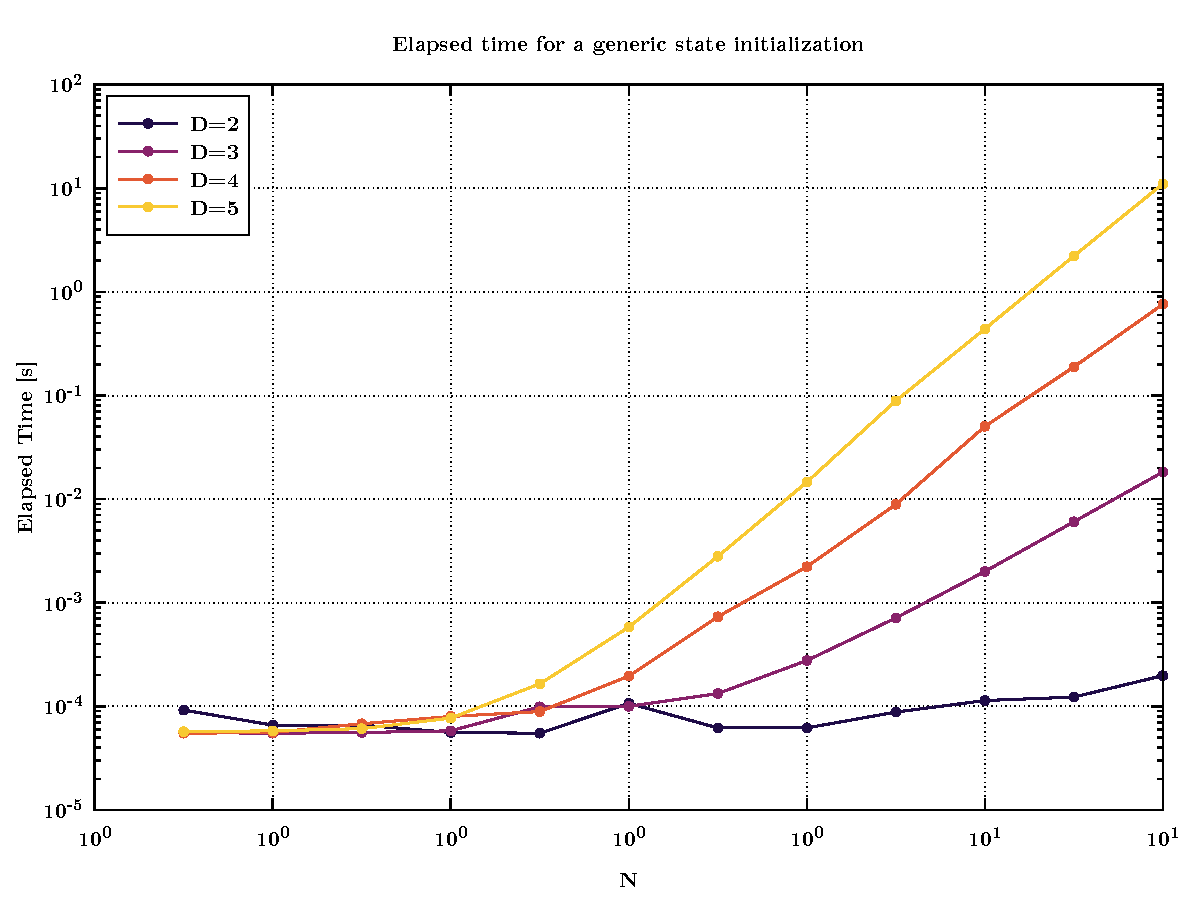
\includegraphics[width=1\textwidth]{image/time_non-sep.pdf}
\end{minipage}
\begin{minipage}[]{0.49\linewidth}
\centering
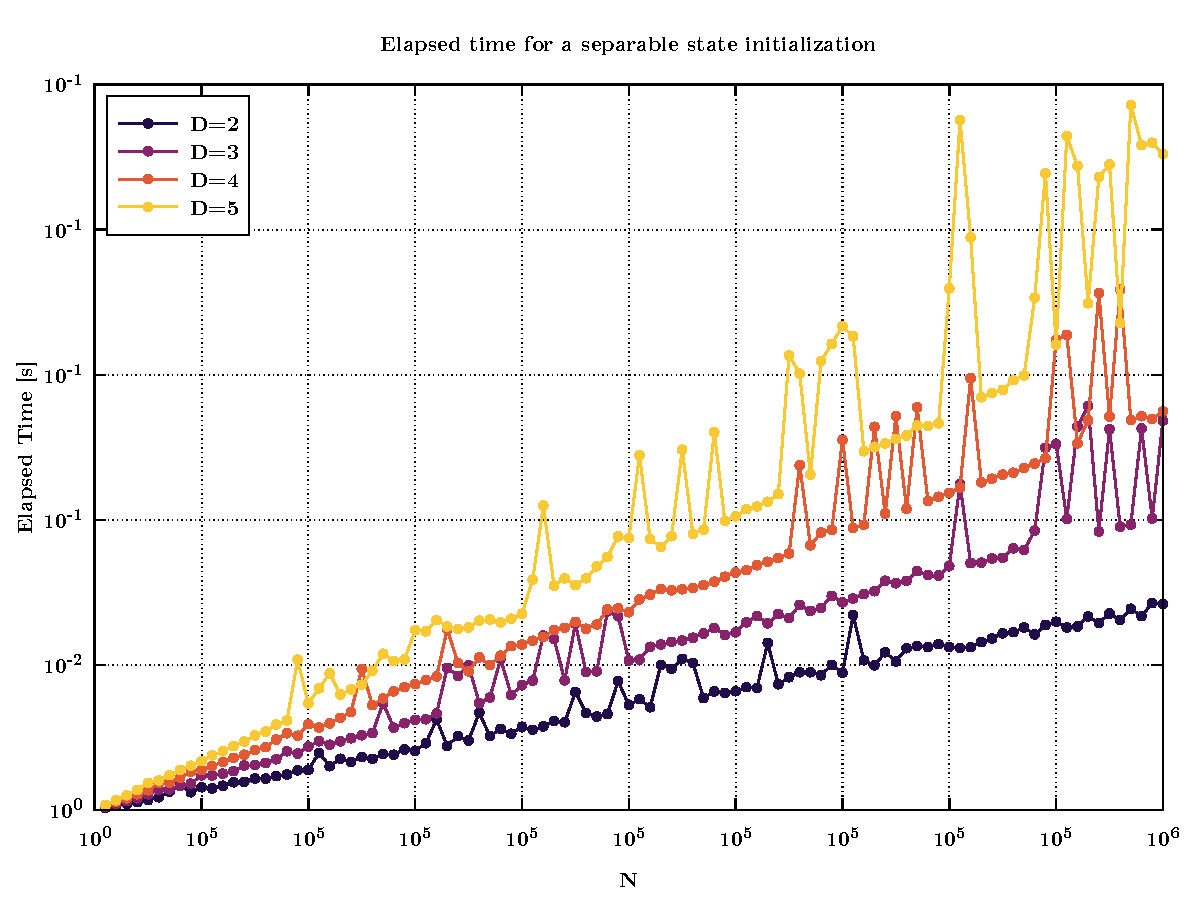
\includegraphics[width=1\textwidth]{image/time_sep.pdf}
\end{minipage}
\caption{\label{fig:init_result} Plot of the computational time required by the function for state coefficients initialization. \textbf{Right:} generic state. \textbf{Left:} separable state.}
\end{figure}

First of all, we test the performance of the subroutine for initializing a quantum state, i.e. finding random coefficients associated to the state. On the right of Fig. \ref{fig:init_result}, we can see the results for a generic state initialization where the initialization of \( D^{N} \) coefficients is required. Instead, on the left, we see the computational time for initializing a separable state where only \( D\times N \) coefficients has to be initialized.
As far as a generic state is concerned, we see that as expected the computational time increases by increasing the space dimension of each subsystem \( D \). For a separable state, we note instability in the curve which can be due to the fact that we are considering short time intervals in which other phenomena influence the execution of the code, such as the computer performance.

After that, we fix \( N=2 \) and we compute the density matrix \( \rho  \) associated to a generic state \( \psi  \). Then, we compute also the reduced density matrix both over the subsystem 1 (\( \rho _1 = \Tr_2 (\rho )  \)) and 2 (\( \rho _2 = \Tr_1 (\rho )  \)).
For instance, starting from a generic two-qubits state (\( D=2 \)):
\begin{equation*}
    \psi =
  \begin{pmatrix}
       0.531654 +0.454865\,i \\
      -0.041827 -0.181760\,i \\
      -0.428231 -0.055035\,i \\
      -0.515319 -0.153920\,i \\
  \end{pmatrix}
\end{equation*}
we compute the following density matrix:
\begin{equation*}
    \rho =
  \begin{pmatrix}
       0.489558 -0.000000\,i & -0.104914 +0.077608\, i & -0.252704 -0.165528\, i & -0.343984 -0.152569\, i \\
      -0.104914 -0.077608\,i &  0.034786 +0.000000\,i &  0.027915 +0.075533\,i &  0.049531 +0.087226\,i \\
      -0.252704 +0.165528\,i &  0.027915 -0.075533\,i &  0.186410 -0.000000\,i &  0.229147 -0.037553\,i \\
      -0.343984 +0.152569\,i &  0.049531 -0.087226\,i &  0.229147 +0.037553\,i &  0.289245 +0.000000\,i
  \end{pmatrix}
\end{equation*}
The obtained reduced matrices are:
\begin{equation*}
    \rho _1 =
  \begin{pmatrix}
    0.675968 -0.000000\,i & 0.124233 +0.040055\,i \\
    0.124233 -0.040055\,i & 0.324032 +0.000000\,i
  \end{pmatrix},
  \qquad \rho_2 =
  \begin{pmatrix}
     0.524344 -0.000000\,i & -0.203173 -0.078301\,i \\
    -0.203173 +0.078301\,i &  0.475656 -0.000000\,i
  \end{pmatrix}
\end{equation*}
These results are in accordance with the theory, since we have that the diagonal entries of \( \rho  \), \( \rho _1 \) and \( \rho _2 \) are real numbers.



\section{Self-evaluation}
The code implemented works well and returns the results expected from the theory. We have seen how initialiazing a separable state can be faster than a generic one.
In a further implementation of the code, it could be useful to compute the density matrix also for a separable state. For doing that, it is needed to recast the \( D\times N \) coefficients into a state.









\end{document}
